\documentclass[main.tex]{subfiles}
\usepackage[utf8]{inputenc}
\usepackage[
backend=biber,
style=alphabetic,
sorting=ynt
]{biblatex}


\addbibresource{references.bib} %Imports bibliography file


\title{Decisión de tipo de residuo}
\author{Rocío Mena}
\date{\today}

\begin{document}

\maketitle

\section{Comparación de Tipos de Residuos para la Economía Circular}

En el marco del desarrollo sostenible, la selección del tipo de residuo a manejar en proyectos de economía circular es crucial. Esta decisión no solo afecta la viabilidad del proyecto \cite{baralla2023waste} sino también su impacto ambiental y social. A continuación, se evalúan diferentes tipos de residuos, destacando sus ventajas y desventajas, para determinar cuál podría ser más apropiado para centrar los esfuerzos de recuperación y reciclaje. \ref{fig:waste-latam}

\begin{figure}[h]
	\centering
	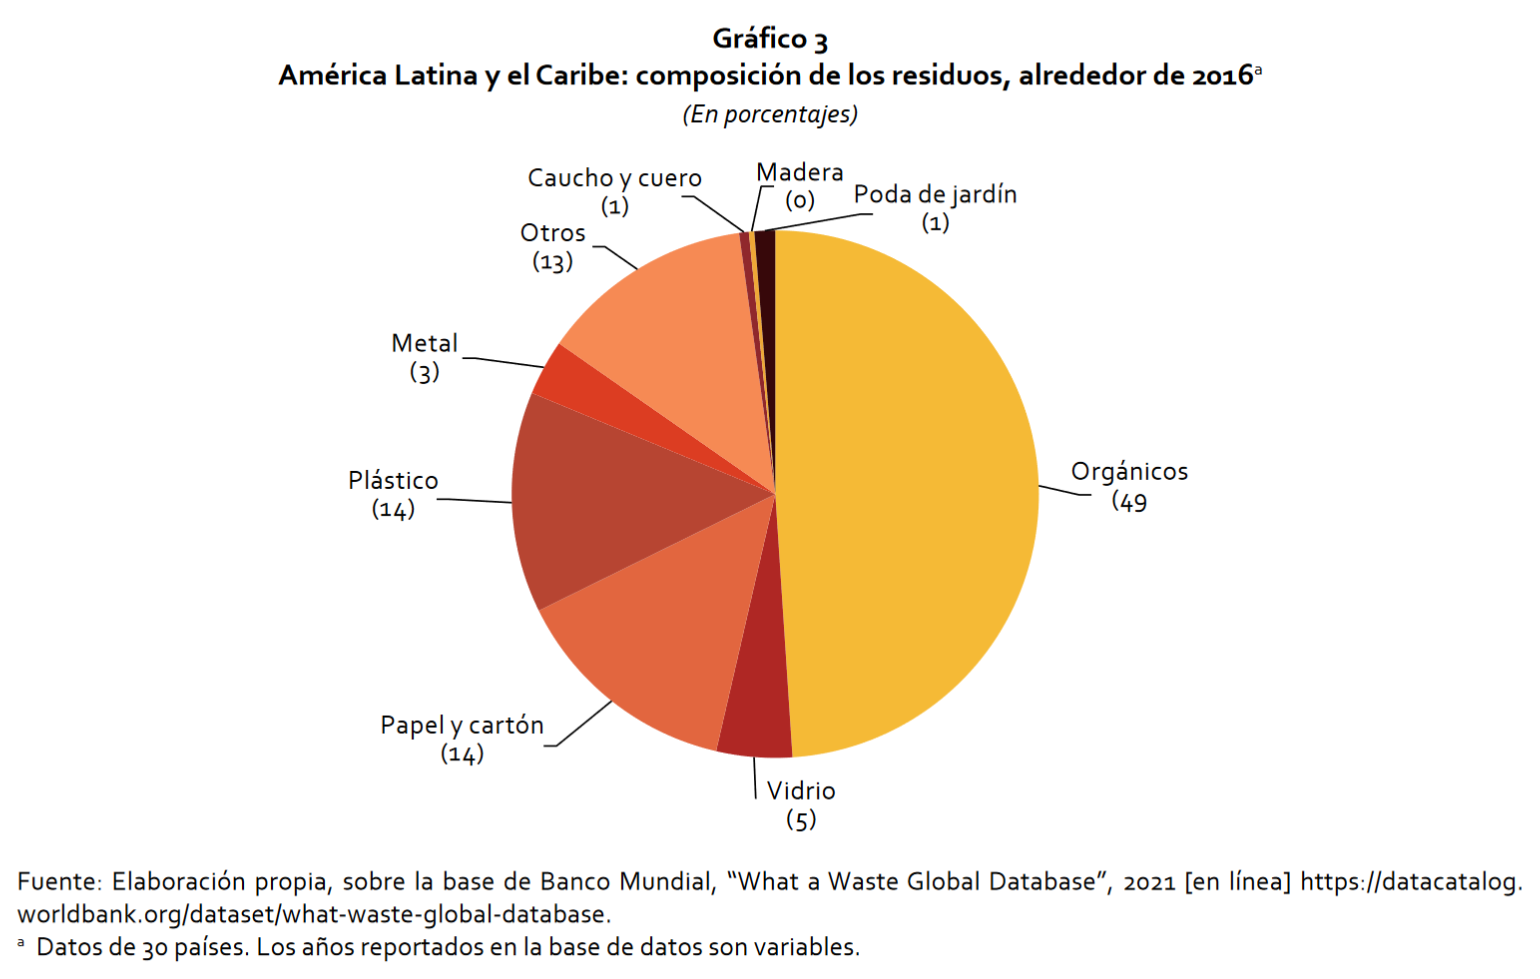
\includegraphics[width=1\textwidth]{./assets/waste-types-latam.png}
	\caption{Composición de los residuos sólidos urbanos en América Latina. Fuente: CEPAL, 2021.}
	\label{fig:waste-latam}
\end{figure}

\subsection{Residuos Orgánicos}
Los residuos orgánicos, como desechos de alimentos y residuos de jardinería, presentan oportunidades significativas para el compostaje y la producción de biogás. Sin embargo, su descomposición produce metano, un potente gas de efecto invernadero, si no se gestiona adecuadamente.

\subsection{Residuos Electrónicos}
Los residuos electrónicos contienen metales preciosos y ofrecen oportunidades económicas significativas. No obstante, su reciclaje presenta desafíos debido a la presencia de sustancias tóxicas, lo que requiere procesos de reciclaje especializados y costosos.

\subsection{Papel y Cartón}
El papel y el cartón son materiales reciclables y biodegradables, lo que los convierte en una opción sostenible. Sin embargo, la calidad del papel reciclado puede ser inferior a la del papel virgen, lo que limita su reutilización en ciertas aplicaciones.

\subsection{Plásticos}
El reciclaje de plásticos puede reducir la dependencia de los recursos fósiles y disminuir la contaminación. Sin embargo, la variedad de tipos de plástico y la contaminación cruzada pueden complicar los procesos de reciclaje, haciéndolos menos eficientes.

\subsection{Textiles}
El reciclaje de textiles apoya la sostenibilidad en la industria de la moda. A pesar de esto, la rápida moda contribuye a altas tasas de desechos textiles, y muchos de estos no son reciclables debido a mezclas de materiales y tratamientos químicos.

\subsection{Metales}
Los metales son altamente reciclables y su recuperación es eficiente en términos de energía. La principal desventaja es la posible degradación de la calidad con ciertos metales no ferrosos, lo que puede limitar su reutilización.

\subsection{Vidrio}
El vidrio es completamente reciclable y puede ser procesado infinitas veces sin pérdida de pureza o calidad. Sin embargo, la recolección y el transporte del vidrio deben manejarse con cuidado para evitar la contaminación y garantizar la viabilidad del reciclado.

Para ser reciclado, el vidrio debe ser separado por color y tipo, lo que puede ser un desafío en la gestión de residuos. Sin embargo, el vidrio reciclado tiene un alto valor en el mercado y puede ser utilizado para fabricar nuevos envases.

\subsection{Residuos de Construcción y Demolición}
Estos residuos ofrecen un gran potencial de reutilización y reciclaje. El principal reto es la separación efectiva de los materiales en el sitio de demolición, lo cual es esencial para su posterior procesamiento.

\subsection{Decisión Final}
Para el alcance de este proyecto, se considerará entre plástico y vidrio debido a su relevancia (14\% y 5\% de la composición de residuos sólidos urbanos en América Latina, respectivamente) y potencial para la implementación de prácticas de economía circular. Se descarta la opción de residuos orgánicos debido a su alta generación de metano y la de residuos electrónicos por su complejidad en el reciclaje. Se descartan también textiles, metales y residuos de la construcción por su menor presencia en la composición de residuos sólidos urbanos en la región. Se descarta papel y cartón por su menor potencial de innovación en comparación con plástico y vidrio.
Se realizará un análisis más profundo de estos dos materiales para determinar cuál de ellos ofrece mayores beneficios y posibilidades de implementación efectiva en el contexto local.

\section{Comparación entre Vidrio y Plástico}

Para una adecuada selección de materiales en proyectos de economía circular, es crucial comprender las diferencias entre los tipos de residuos más comunes. A continuación se presenta una comparación detallada entre vidrio y plástico basada en varios criterios importantes para su gestión y reciclaje.

\begin{table}[h!]
\centering
\begin{tabular}{|l|c|c|}
\hline
\textbf{Criterio} & \textbf{Vidrio} & \textbf{Plástico} \\ \hline
Cantidad generada & 5\% & 14\% \\ \hline
Variedad de tipos & Baja & Alta \\ \hline
Usos comunes & Envases, ventanas, vajillas & Envases, muebles, electrónica \\ \hline
Complejidad de reciclaje & Baja & Alta \\ \hline
Impacto ambiental & Menor & Mayor \\ \hline
Tasa de reciclaje & Alta & Variable, generalmente baja \\ \hline
Degradación por reciclado & No degrada & Degradación de calidad \\ \hline
Requerimientos de tratamiento & Fundición a alta temperatura & Diversos métodos según tipo \\ \hline
Potencial de mercado para reciclados & Estable & Creciente pero complejo \\ \hline
\end{tabular}
\caption{Comparación entre vidrio y plástico en el contexto de economía circular.}
\label{tab:glass-vs-plastic}
\end{table}

Como se puede observar en la tabla \ref{tab:glass-vs-plastic}, el vidrio y el plástico presentan diferencias significativas en términos de cantidad generada, variedad, usos, y complejidad en su reciclaje. Mientras que el vidrio tiene una tasa de reciclaje relativamente alta y un impacto ambiental menor debido a su capacidad de ser reciclado múltiples veces sin pérdida de calidad, el plástico, aunque más versátil y utilizado en una variedad más amplia de productos, enfrenta desafíos significativos debido a su alta variedad y la degradación de calidad con cada ciclo de reciclado. Además, el impacto ambiental del plástico es considerablemente mayor, especialmente por su contribución a la contaminación marina y la dificultad de descomposición.

Debido a estas características, dentro del alcance de este trabajo se elige el vidrio como el material principal para la implementación de prácticas de economía circular en el contexto local. A pesar de su menor presencia en los residuos sólidos urbanos, el vidrio ofrece ventajas significativas en términos de reciclaje, impacto ambiental y viabilidad de mercado para los reciclados. 

El reciclaje del vidrio resulta de particular importancia local en Mendoza, donde la industria del vino es una actividad económica clave y el vidrio es un material esencial en la cadena de suministro de vino. A su vez, en la provincia se encuentra radicada la fábrica nacional de Vidrios de Verallia Argentina, una de las principales empresas de fabricación de envases de vidrio en el país. Esta empresa es un actor clave en la cadena de suministro de vidrio y su participación en iniciativas de economía circular puede tener un impacto significativo en la sostenibilidad de la industria del vino y en la economía regional. A su vez, esta empresa actualmente ya cuenta con prácticas de reciclaje de vidrio, lo que facilitaría la implementación de nuevas tecnologías y procesos para mejorar la trazabilidad y la gestión de residuos en la cadena de suministro.

A lo largo de este trabajo se realizará un análisis más detallado de la cadena de suministro del vidrio y las oportunidades de innovación en el reciclaje de vidrio para maximizar su potencial en la economía circular.

\end{document}
